\begin{figure*}[!htbp]
    \centering
    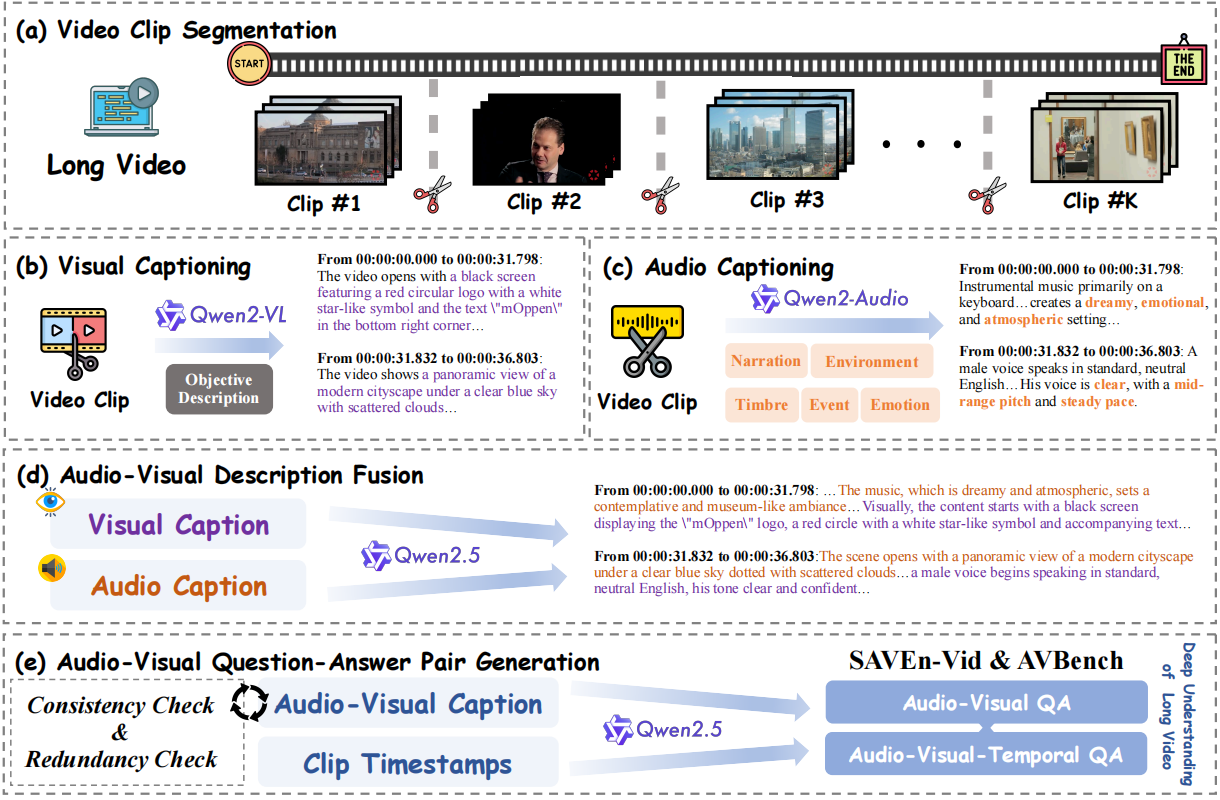
\includegraphics[width=\textwidth]{figures/2_longAV_pipeline_.pdf}
    \caption{\textbf{Overview of the \OurDataset{} construction pipeline.} (a) Employ the AutoShot model to perform \textbf{Video Clip Segmentation} on the original long video. (b) Utilize the Qwen2-VL model to perform \textbf{Visual Captioning}. (c) The \textbf{Audio Captioning} using the Qwen2-Audio model, which not only provides explicit sound descriptions of objects or events but also delves into indirect information conveyed by sounds, such as their source, sound quality, and emotional hues. (d) Leverage the Qwen2.5 model to perform \textbf{Audio-Visual Description Fusion}, forming comprehensive audio-visual descriptions at the segment level. (e) Reapply the Qwen2.5 model to execute \textbf{Audio-Visual Question-Answer Pair Generation}, consistency checks and detect redundant content.}
    % 完备版:(a) 首先,采用AutoShot对原始长视频进行视觉语义分割,将其分解为具有独立意义的视频片段。这一过程基于视频内容的视觉特征,确保每个分割出的片段都具有明确的主题或场景转换。(b) 接着,利用Qwen2-VL模型对这些视频片段进行细粒度的视觉内容标注。此模型能够提供详尽的图像描述,包括但不限于人物、物体、动作及场景细节,从而丰富了视频内容的信息量。(c) 同时,针对视频中的音频部分,我们运用Qwen2-Audio模型进行细粒度的声学特征分析。这不仅涵盖了对显性物体或事件的声音描述,还深入挖掘了声音的间接信息,如声源性质、音质特点、背景环境以及情感色彩等,以全面捕捉音频数据的多维度信息。(d) 在获取到视频和音频的详细描述后,我们借助Qwen2.5模型将两者的信息进行有效融合,形成片段级别的综合描述。(e) 接下来,为了保证信息的准确性和连贯性,我们再次利用Qwen2.5模型执行了一致性校验,识别并修正了可能存在的错误标签。此外,模型还进行了冗余内容检测,有效地精简了重复或无关紧要的信息,进一步优化了文本的质量。最终,通过Qwen2.5模型整合各个片段的描述,构建了一个连贯且全面的视频整体叙述,实现了从局部描述到整体故事的无缝衔接。基于这些高质量的文本描述及其对应的时间戳,我们生成了一系列精准的问答对。
    % 精简版:(a) 使用AutoShot对原始长视频进行视觉语义分割,确保每个片段有明确的主题或场景转换。(b) Qwen2-VL模型对视频片段进行细粒度的视觉内容标注,包括但不限于人物、物体、动作及场景细节。(c) Qwen2-Audio模型分析视频中的音频,不仅涵盖了对显性物体或事件的声音描述,还深入挖掘了声音的间接信息,如声源性质、音质特点、背景环境以及情感色彩等(d) 利用Qwen2.5模型融合视听信息,形成片段级别的综合视听描述。(e) 再次使用Qwen2.5模型执行一致性校验和冗余内容检测,整合各片段描述,构建连贯的视频叙述,最终使用Qwen2.5模型生成问答对。
    \label{fig:ds_pipline}
\end{figure*}